\section{Introduction}
\begin{figure*}[h]
	\centering
	\subfigure[Age]{
		\centering
		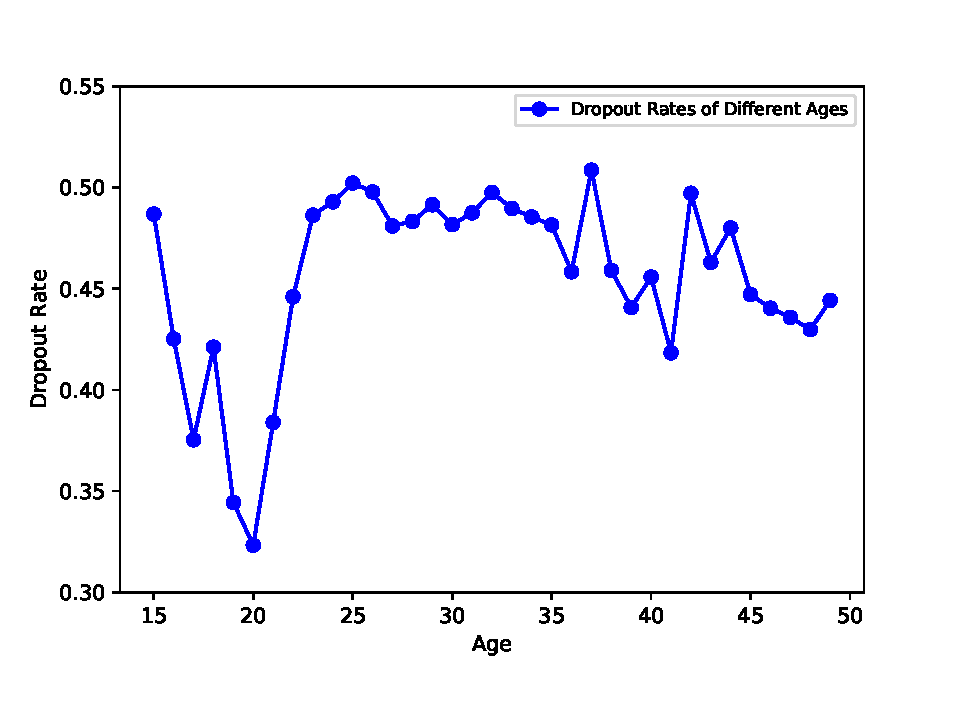
\includegraphics[height=1.69in]{age_dropout.pdf}}%
	\subfigure[Course Category]{
		\centering
		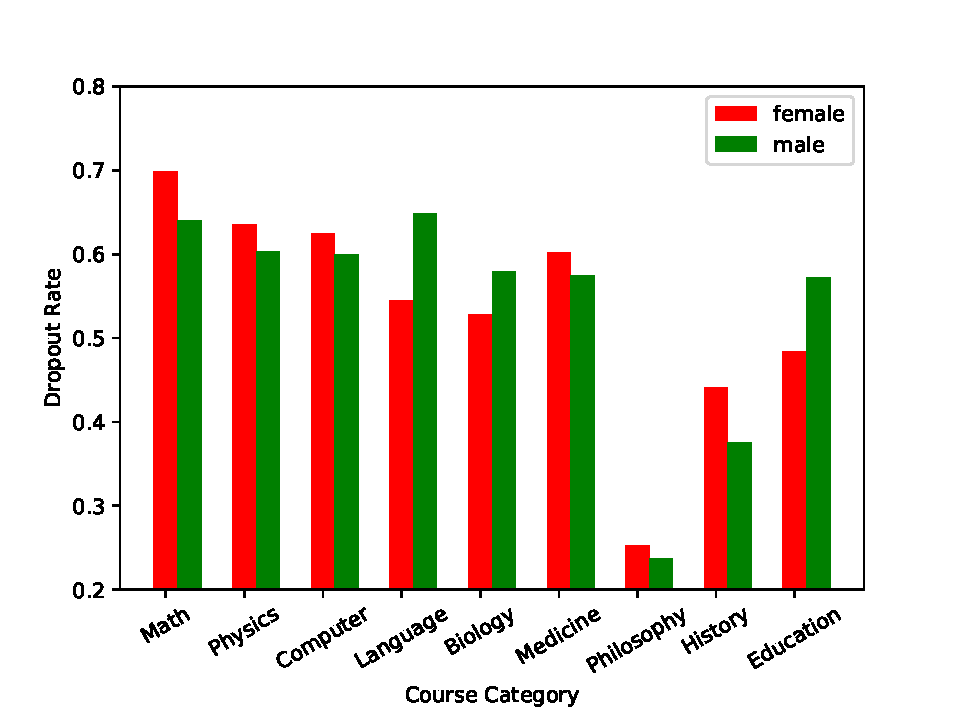
\includegraphics[height=1.7in]{gender_category_prune_2.pdf}
	}
	\subfigure[Education Level]{
		\centering
		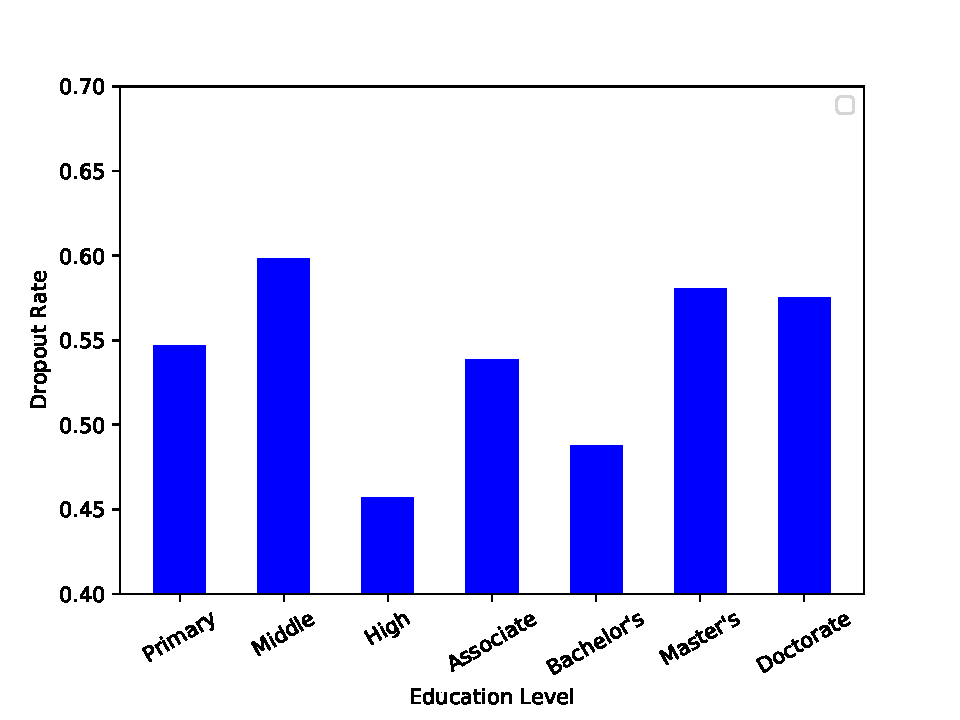
\includegraphics[height=1.7in]{education_stat_prune.pdf}
	}
	%\vspace{-0.1in}
	\caption{Dropout rates of different demographics of users. (a) user age (b) course category (c) user education level.}%. $Y$-axis: dropout rate of users} 
	\label{fig:dropStat} %% label for entire figure 
\end{figure*}

%As a new type of education method, m
% since it appeared in 2012 
%. 
%and XuetangX in China. 
%from more than 800 universities~\cite{shah2018product}. 
Massive open online courses (MOOCs) have become increasingly
popular.
Many MOOC platforms have been launched. For example, Coursera, edX, and Udacity are three pioneers, followed by many others from different countries such as 
XuetangX in China, Khan Academy in North America, Miriada in
Spain, Iversity in German, FutureLearn in England, Open2Study
in Australia, Fun in France, Veduca in Brazil, and Schoo in Japan~\cite{Qiu:2016:MPL:2835776.2835842}.
By the end of 2017, the MOOC platforms have offered 9,400 courses worldwide and attracted 81,000,000 online registered students~\cite{shah2018product}. 
Recently, a survey from Coursera shows that MOOCs are really beneficial to the learners who \textit{complete} courses, where 61\% of survey respondents report MOOCs' education benefits and 72\% of those report career benefits~\cite{zhenghao2015s}. 
%: 61\% of  report MOOCs' educational benefits and 72\% feed back that MOOCs boost their careers. 
%Many MOOCs platforms have been launched up to now, such as Coursera, edX, Udacity, and XuetangX in China.
%Apart from overturning the traditional model of higher education,

However, on the other hand, MOOCs are criticized for the low completion ratio~\cite{He:2015:IAS:2886521.2886563}. 
Indeed, the average course completion rate on edX is only 5\%~\cite{Kizilcec:2013:DDA:2460296.2460330,Seaton2014Who}.
We did a similar statistic for 1,000 courses on XuetangX, and resulted in a similar number --- 4.5\%.
% we find that nearly 79\% users drop out from their enrolled courses. 
\hide{
Meanwhile, the success of MOOCs greatly promote scientific research on education \cite{article,Crow2013}. One of the most urgent research topics is dropout prediction in MOOCs \cite{He:2015:IAS:2886521.2886563}, because of the substantially higher dropout rates on MOOCs than that of traditional education\cite{Clow:2013:MFP:2460296.2460332}, e.g. the average course completion rate on Edx is only 5\% \cite{Kizilcec:2013:DDA:2460296.2460330,Seaton2014Who} and using statistics from over 1000 courses on XuetangX, we find that nearly 79\% users drop out from their enrolled courses. 
}
%Some people argue that the main possible reason for the high dropout rate on MOOCs might be the low monetary cost, i.e., most MOOCs courses are free.
%Some other people state that motivations of the users to study online very differently.
Figure \ref{fig:dropStat} shows several observational analyses. As can be seen, Age is an important factor --- young people are more inclined to drop out; Gender is another important factor --- roughly, female users are more likely to drop science courses and male users are more likely to give up non-science courses; finally, educational background is also important. 
This raises several interesting questions: 1) what are the major dropout reasons? 2) what are the deep motivations that drive the users to study or induce them to drop out?
3) is that possible to  predict users' dropout behavior in advance, so that the MOOCs platform could deliver some kind of useful  interventions~\cite{halawa2014dropout,Qi:18NIPS}?

%, and social pressure for dropping out a course is limited as most MOOCs users take the course online by themselves, while in the traditional classroom setting, students suffer from social pressure when they drop out a course. Therefore, identifying users who have risk of dropout and taking efficient interventions to hold back them is really necessary for MOOC platforms. 
%Furthermore, analyzing individual learning behavior and predicting their likelihood of dropout in a real-time dynamic way can also enhance students learning on MOOCs\cite{halawa2014dropout}. 

%This can help  In the short-run, this can help help instructors to identify users that are in need of scaffolding, and to deliver interventions to help them. In the long term, dropout prediction and analysis can provide valuable insights into the interactions between course design and student factors.  

%dropout analysis and prediction in MOOCs are extremely significant, which would offer both short-term and long-term value\cite{halawa2014dropout}: In the short term, predicting dropout can help instructors to identify users that are in need of scaffolding, and to deliver interventions to help them. In the long term, dropout prediction and analysis can provide valuable insights into the interactions between course design and student factors.
\hide{
In this paper, we focus on studying users' dropout behavior in MOOCs. More specifically, we aims to answer three questions: How to identify dropout reasons of users? How to predict who or when drops out? How to retain users with high risk of dropout in a course? Though several related work, such as user engagement analysis \cite{Anderson:2014:EMO:2566486.2568042ß}, learning behavior prediction\cite{Qiu:2016:MPL:2835776.2835842} and dropout prediction \cite{Nagrecha:2017:MDP:3041021.3054162}, few researches have explored above questions systematically for large scale MOOC learners.

The main challenge to solve theses questions is the diversity of students in MOOCs. Since MOOCs are accessible towards anyone around the world, students in MOOCs have much more diverse background(such as age, education level, location and so on) than those in the traditional classroom. Consequently, their engagement and learning behavior exhibit much more heterogeneity, which further causes different trends of dropout. Our preliminary studies(in Figure \ref{fig:dropStat}) show that different demographics of users in XuetangX exhibits quite different level of dropout rates. However, the data which enable us to learn individual preference for a specific type of users is quite sparse, which causes the difficulty of understanding their dropout motivation and training a personalized dropout prediction model.
}

%In this paper, e%By employing XuetangX, one of the largest Chinese MOOC platforms, as our research source, we 
Employing a  dataset from XuetangX, the largest MOOC platform in China, we aim to conduct a systematical exploration for the aforementioned questions. 
We first perform a clustering analysis over users' learning activity data and found that  users' studying behavior can be grouped into several categories, which implicitly correspond to different motivations that users study MOOC courses.
The analyses also disclose several interesting patterns. 
For example, the dropout rates between similar courses is highly correlated;
friends' dropout behaviors strongly influence each other ---
the probability that a user drops out from a course increases quickly to 65\% when the number of her/his dropout friends increases to 5.

%monotonically from 0.33 to 0.87 when their dropout friends increases from 0 to 10.

\hide{
We first propose a simple but effective method to cluster users based on their temporal engagement patterns, which helps understand users' complex engagement patterns on MOOCs. Furthermore, we conduct statistical analyses to identify potential factors(including co-learning courses and dropout friends(co-learning users))  that affect users' dropout. We have several useful discoveries in this stage. First, we observe that students with lower dropout rate always exhibit higher learning efficiency on course contents and higher correct ratio on homework. Second, dropping out from a course has a positive and significant correlation with dropping out from other co-learning courses. Third, dropout friends indeed have an important influence on users' dropout. The probability that users drop out from their courses increases monotonically from 0.33 to 0.87 when their dropout friends increases from 0 to 10.
}
%Context-aware Feature Interaction Network (CFIN) to 
Based on the analyses results, 
we propose a Context-aware Feature Interaction Network (\modelname{}) to
model and to predict users' dropout behavior. 
In \modelname{}, we utilize a context-smoothing technique to 
smooth values of activity features  using the convolutional neural network (CNN).
%to fuse the information learned from different sources.
Attention mechanisms are then used to combine user and course 
information into the modeling framework.
We evaluate the proposed \modelname{} on two datasets: KDDCUP and XuetangX. The first dataset was used in KDDCUP 2015 and the second one is larger, extracted from the XuetangX system.
Experiments on both datasets 
show that the proposed method achieves much better performance than several state-of-the-art methods. 
We have deployed the proposed method in XuetangX to help improve user retention.

\hide{we then design an algorithm framework to extract a rich set of effective features to capture both activity features and personalized information for each user. Moreover, we utilize deep learning methods, i.e., LSTM and network embedding, to learn latent features from users' activities and social information, which further improve the prediction performance. To assemble these diverse features, we propose a semi-supervised co-training framework to predict users' dropout. By leveraging unlabeled data, this framework can alleviate the sparsity problem. The method achieves \textbf{90.93\%} AUC score on the dataset provided by KDDCUP 2015, which is comparable to the winner team's methods of this competition. We also conduct offline experiments on the large-scale dataset from XuetangX. Our method achieves \textbf{3.14-3.50}\% AUC improvement compared to basic linear classification methods. Furthermore, our framework has been deployed by XuetangX, and facilitating over 10,000,000 registered users retention. 
}
%Figure ? shows our preliminary study for the dropout rates of users of different profiles in XuetangX.  
%However, the information which enables us to identify a particular MOOCs user's background is very limited, which causes the difficulty of understanding her motivation for dropout. 
%Unlike the traditional classroom, MOOCs are accessible towards anyone around the world. Thus MOOCs students have more diverse background. 
%Despite of the importance of predicting dropout rate, it remains substantial difficulty to execute this task accurately. 
%Why, who and when drops out?

%\begin{itemize}
%	\item Since MOOCs are accessible towards anyone around the world, MOOCs students have much more diverse background than those in the traditional classroom. Consequently, their engagement and learning behavior exhibit much more heterogeneity, which further causes different level of dropout rate. However, the information which enables us to identify a particular MOOCs user's background is very limited, which causes the difficulty of understanding her motivation for dropout. 
    %This results in the diverse causes of dropout furthermore. 
   % For an individual user, we don't know who he is and why he comes or drops from MOOCs.
 %   \item  Our analyses show that about 68\% users only enroll in one course on XuetangX. Thus, both the enrollment and log data for a specific user can be rather sparse, and this leads to insufficient training data to learn a user's individual information and to predict her dropout likelihood.
%    \item Since there are numerous underlying factors that are related to a user's dropout behavior on MOOCs, such as user demographics, course categories, and social factors, it is difficult to incorporate all these factors into one unified model for dropout prediction. 
%\end{itemize}


	%We address these challenges as follows. 
%	\textbf{First}, we conduct statistical analyses to identify potential causes that affect users' dropout, and propose a simple but effective method to cluster users based on their temporal engagement patterns, which helps understand users' complex engagement patterns on MOOCs. 
%	\textbf{Second}, based on aforementioned analyses results, we design an algorithm framework to extract a rich set of effective features to capture both activity features and individual information for each user. Moreover, we utilize deeplearning methods, i.e., LSTM and network embedding, to learn latent features from users' activities and user enrollment information, which further improve the prediction performance.
%	 \textbf{Last but not least}, we propose a semi-supervised co-training framework to predict users' dropout via combining these diverse features. By leveraging unlabeled data, this framework can alleviate the sparsity problem.
	



